\documentclass[a4paper , 12pt]{article}


\usepackage[utf8]{inputenc}
\usepackage{fancyhdr}
\usepackage{geometry}
\usepackage[frenchb]{babel}
\usepackage{libertine}
\usepackage[pdftex]{graphicx}
\usepackage{hyperref}
\usepackage{slashbox}
\usepackage[T1]{fontenc}
\usepackage{multirow}
\usepackage{graphicx}
\usepackage{array,multirow,makecell}
\setcellgapes{1pt}
\makegapedcells
\newcolumntype{R}[1]{>{\raggedleft\arraybackslash }b{#1}}
\newcolumntype{L}[1]{>{\raggedright\arraybackslash }b{#1}}
\newcolumntype{C}[1]{>{\centering\arraybackslash }b{#1}}
\geometry{a4paper}
\geometry{top=3cm, bottom=2.5cm, left=4cm, right=3cm}

\renewcommand{\baselinestretch}{1.5} 

\begin{document}


\begin{titlepage}
\begin{centering}
		\title{Rapport de projet InfoSUP EPITA : Lucidity by the Chamallow}
		 
		\author{CLAUS Marion claus\_m -  DELECROIX Thomas  delect\_t - \\GINANE Charles ginane\_c - 
 MARCHAUD Laurent marcha\_4} 

\end{centering}
\end{titlepage}
\pagestyle{fancy}
\lhead{The Chamallow}
\rfoot{EPITA infosup}
\renewcommand{\footrulewidth}{0.4pt}
\rhead{Rapport de projet}

  \begin{titlepage}
\centering
\maketitle

	
\includegraphics[scale=0.1]{Logo.png}

  \end{titlepage}

\newpage

\tableofcontents

\newpage

\begin{flushleft}

\large

\textbf{Table des illustrations :}

\end{flushleft} 

\quad

- Figure 1 : Tableau de répartitions des tâches, tableau : Page 14

\quad

- Figure 2 : Tableau d'avancement du projet par soutenance, tableau : page 15

\quad

- Figure 3 : Checkpoints, capture d'écran : Page 24

\quad

- Figure 4 : HUD, capture d'écran : page 28

\quad

- Figure 5 : Le menu options, capture d'écran : page 29

\quad

- Figure 6 : Modification du son "pas", capture d'écran : page 33

\quad

- Figure 7 : Page d'accueil de notre site, capture d'écran : page 34

\quad

- Figure 8 : Porte présente dans nos niveaux, capture d'écran : Annexe

\quad

 - Figure 9 : Une plateforme automatique, capture d'écran : Annexe

\quad

- Figure 10 : Une plateforme contrôlée par des clips, capture d'écran: Annexe

\quad

- Figure 11 : Bouton présent dans le niveau 2 du solo , capture d'écran : Annexe



\newpage



\section{Introduction}

\quad

Nous allons enfin pouvoir vous présenter la version finale de notre projet de Sup : Lucidity. Il nous a demandé un travail considérable mais nous y sommes arrivés à bout. Ce rapport de projet vous décrira l’avancement de notre jeu, du début de sa conception jusqu’à sa finalisation, ainsi que notre découverte du travail d’équipe.\\

    Ce projet a permis de passer des bons moments, ainsi que d’autres moins bons mais cela reste une expérience enrichissante que nous serions tous prêts à refaire. Vous pourrez découvrir tout cela au fil des pages.\\

    Tout d’abord nous vous présenterons le scénario de notre jeu, ainsi qu’une reprise du cahier des charges qui présente le groupe et le jeu. Vous pourrez ensuite découvrir l’avancement de ce dernier au fil des soutenances, puis les tâches respectives de chaque membre. Il y aura ensuite un bilan sur ce que chaque membre du groupe a pensé de ce projet, suivi de nos problèmes et de nos joies et pour finir la webographie.



\quad

\newpage

\section{Scénario du jeu}

\quad

En 3042, les scientifiques du monde entier se sont unis pour pouvoir partager toutes les connaissances accumulées au cours des siècles. Ainsi ils ont pu faire beaucoup de progrès, surtout dans le domaine spatial. Cela a permis à l’espèce humaine de commencer à coloniser l’espace. D’abord des planètes viables près de la planète Terre, puis de plus en plus loin, jusqu’à aller dans d’autres galaxies. Maintenant, ils ont commencé à coloniser une nouvelle galaxie, très très lointaine. Dans cette galaxie, des humains se sont installés sur une planète qu’ils ont appelée Lucidios. Cette planète est complètement différente de la Terre. Là-bas, ils ont trouvé des matériaux qui n’existent sur aucune des planètes déjà colonisées, ils ont aussi découvert un liquide multicolore qu’ils ont décidé de nommer la Lucidité.\\

Assez intrigués par cette dernière, des scientifiques ont fait des recherches dessus et après certains tests. Ils pensent que l’on pourrait l’utiliser comme une ressource dans la vie quotidienne des lucidiociens. Par exemple, en permettant de se déplacer d’un endroit à un autre en utilisant des plateformes mais aussi des portails. Effectivement, les scientifiques espèrent utiliser la Lucidité comme une source d’énergie. Ainsi en la mettant dans un mécanisme, cela permettrait d’actionner ce dernier. \\

Pour finaliser les tests, des salles ont été créées dans lesquelles il y a des objets avec lesquels il est possible d’interagir grâce à la Lucidité. Ils sont donc à la recherche de volontaires dont la mission sera de traverser ces salles en transportant de la Lucidité en bouteille. Le problème c’est qu’ils auront donc un stock limité sur eux, ils devront donc apprendre à maîtriser cette perte de ressource car ils ne pourront remplir leur réserve qu’au niveau de source de Lucidité. S’ils arrivent à traverser toutes les salles qui contiennent  des tests de difficulté croissante, leur mission sera réussite et ils pourront l’utiliser sur toute la planète et peut-être même sur les planètes voisines. Si vous êtes volontaire, n’hésitez pas à vous rendre sur notre site internet “lucidity.fr” pour vous inscrire.

\newpage

\section{Récapitulatif du cahier des charges}

\subsection{Présentation du groupe et du projet}

	\subsubsection{Présentation du groupe}

\quad

	\underline{\textbf{Le groupe en lui même :}}

\quad

    Notre groupe composé de Thomas “Tetra” DELECROIX, Charles “Gigi” GINANE, Marion “Santa” CLAUS et Laurent “Aluxima” MARCHAUD provient de la classe A2. Nous nous sommes mis ensemble dans l’optique de créer un groupe d’un niveau homogène.
Son nom provient du début des premières syllabes de nos prénoms: “Tho”, “Cha”, “Ma” et “Lau”, transformé en “The Chamallow”.
 
\quad

	\underline{\textbf{Présentation personnelle de chacun}}

\quad

		\underline{Thomas "Tetra" DELECROIX }
			
L’an dernier j’étais en terminale S en spécialité informatique et sciences du numérique. J’ai déjà quelques connaissances sur certains langages de programmation, mis à part le CAML, Csharp et Python que nous avons traités pendant ce premier semestre à Epita, comme en HTML, JavaScript, CSS, ActionScript et un peu de domotique avec Arduino. Pour notre groupe ce projet va nous apprendre à travailler en groupe ainsi que communiquer entre nous. Personnellement ce projet va sûrement me permettre d'approfondir ma méthodologie, mon analyse, ma réflexion ainsi que mes connaissances dans des langages comme par exemple le Csharp. Etant chef de groupe je vais également avoir la responsabilité de la cohésion et la motivation du groupe ainsi que du respect des deadlines que nous nous fixons.

\quad

\newpage

		\underline{Marion "Santa" CLAUS}
			
\quad

Contrairement à une bonne majorité des étudiants d’EPITA, l’informatique m’intéresse depuis peu de temps. Cela a commencé en terminale quand ma curiosité m’a poussée en spécialité ISN. Ainsi, à mon arrivée à EPITA, j’avais fait un peu de programmation en Python et avais quelques connaissances en HTML. Donc quand j’ai appris que j’allais travailler en groupe pour coder un jeu vidéo, je me suis dit que c’était une opportunité à saisir, que je pourrais apprendre de nouvelles choses. Bien sûr le fait qu’il ait un temps limite fait de ce projet un challenge que je suis prête à relever. Si vous ne l'aviez pas compris, j’aime élargir mes connaissances, c’est pourquoi je m’occuperai essentiellement de la partie graphique, un domaine qui m’est totalement inconnu.

\quad

		\underline{Charles "Gigi" GINANE}
			
\quad

Moi c’est Charles sous le surnom GIGI, je viens de province (du Sud plus exactement) d’une terminale Scientifique spécialité Physique. Par curiosité je me suis intéressé petit à petit à l’informatique à l’âge de 12 ans dès que j’ai eu mon ordinateur personnel.
Par curiosité, j’ai découvert quelques langages informatiques tels que le C, le C++, le php, le html et le css que j’ai pu expérimenter lors des TPE en créant notre propre site internet.
J’ai étendu ma passion en donnant des cours au club informatique de Montélimar ou bien en m’occupant de retransmettre des match de boules lyonnaises sur internet en direct.
Le fait de travailler en groupe est un atout pour moi, je pourrai apprendre des choses que j’ignorais et aussi apporter des connaissances que les autres n’ont pas (notamment en LaTeX !).
L’idée de faire de faire un projet ne me fait pas peur et ce premier projet va m’apporter beaucoup de connaissances car l’entente avec les autres membres du groupe est parfaite.

\newpage

		\underline{Laurent "Aluxima" MARCHAUD}

\quad

Venant de terminale S spécialité informatique et sciences du numérique (ISN), j’ai déjà quelques bases en programmation C/C++, Python, Caml, php et html, acquises en cours ou par curiosité avant le lycée. L’idée de créer un jeu vidéo de A à Z est alors quelque chose qui me motive énormément, notamment dans l’apprentissage du Csharp, le respect de délais, l’organisation et le travail de groupe. Pour le moment, mon seul travail de groupe en informatique a été le projet d’ISN de l’année dernière, que j’ai fait en binôme avec un ami. Tout s’est extrêmement bien passé et nous avons presque décroché la note maximale ! J’espère alors que ce travail se déroulera aussi bien; pour cela il faudra s’impliquer au maximum et ne jamais baisser les bras.
Je m’attends donc à ce que, en un semestre, nous puissions développer un jeu fantastique, complet, et tout ça, bien évidemment, sans aucun bug !

\newpage

\subsubsection{Présentation du projet}

\quad

\underline{Origine}

\quad

En premier lieu, nous n’avions pas d’idée précise sur le jeu que nous allions faire, mais au cours du temps nous avons réussi à éliminer les choix qui ne nous convenaient pas. Nous avons alors retiré les jeux types RPG, RTS, MOBA. L’idée d’un jeu de réflexion/plateforme nous est venue. Nous pensions d’abord faire un jeu de création de mécanismes constitués d’objets du décor, avec l’idée de faire comme, dans le jeu Minecraft, des systèmes de redstone (liaisons de fils et de composants) mais nous y avons réfléchi et avons pensé qu’un tel jeu serait trop ambitieux et que nous n’aurions sûrement pas suffisamment de temps pour terminer ce projet. Nous nous sommes alors restreints à l’interaction avec le décor, tel que des boutons.

\quad


	\underline{Nature}

\quad

    Notre ambition est donc de créer un jeu de réflexion/plateforme/puzzle. La vue du personnage serait à la première personne. L’environnement serait à première vue des sortes de salles closes dans lesquelles le joueur doit effectuer une suite d’actions en interaction avec le décor lui permettant de sortir de la salle et de passer à un niveau supérieur. Notre jeu s'inspirant du principe du jeu de réflexion “Portal”. La ressource primaire (épuisable) du jeu serait la “Lucidité” qui pourrait, par exemple, servir à avoir des interactions à distance avec les objets. Cette ressource serait récoltée en exploitant des sources, rares, présentes à certains endroits de la carte. La lucidité serait contenable en quantité limitée dans une bouteille spéciale que le joueur transportera dans son dos. Le jeu se rapprochant le plus du nôtre est Q.U.B.E. Ce dernier est basé sur la construction de plateformes grâce à des solides physiques comportant des propriétés particulières comme la déformation, l’assemblage, etc.
Cela se traduit par le déplacement d’objets, pression de boutons, déplacements, etc. Il faudra également penser à l’aspect multijoueur du jeu en créant un mode de jeu adapté. Les joueurs évolueront ensemble et devront impérativement s’aider et effectuer des actions ensemble pour finir chaque niveau.

\quad
 
	\underline{Buts et intérêts}

\quad

    Ce projet a pour but de nous initier premièrement au travail de groupe. De plus il nous permettra de découvrir de nouveaux logiciels comme Unity, Blender et d’approfondir nos connaissances en C\#, LaTeX, Php, HTML, et tous les langages que nous rencontrerons.
La programmation de ce jeu induira également l’usage de formules mathématiques et physiques pour l’application de mouvements des objets, des trajectoires, etc.

\newpage

\subsection{Description du projet}

	\subsubsection{Les domaines développés dans ce projet}
Dans cette partie, nous allons vous présenter les differents domaines que nous developperons tout au long de notre projet. En voici la liste :

\quad

- \underline{Moteur Graphique : } Le moteur graphique inclus à Unity va nous permettre d’afficher les differentes structures visuelles présentes dans notre jeu.

\quad 

- \underline{Moteur Physique : } Ce moteur va permettre de gérer dans notre projet tout ce qui est collision entre le joueur et les murs, l’attraction de certains objets, la gravité dans le monde, le déplacement du personnage et des objets.

\quad

- \underline{Site : } Nous allons créer un site web sur lequel nous mettrons une présentation du projet et des membres du groupe, l’avancement du projet, comment nous contacter, des captures d’écran du jeu et les liens de nos sources. Il y aura aussi une version téléchargeable du jeu et un moyen pour s’inscrire/se connecter au jeu.

\quad

- \underline{Reseau : } Le réseau nous est nécessaire puisque nous avons l’ambition de faire un multijoueur ce qui nous oblige à adapter notre jeu.

\quad

- \underline{Gameplay : } Le gameplay est obligatoire dans tout jeu afin que le jeu soit jouable par une grande partie du public, c’est pour cela que nous le developperons et l’adapterons au cours de ce projet.

\quad

- \underline{Conception du monde : } Nous comptons créer différentes salles de difficultés différentes auquelles le ou les joueurs seront confrontés afin de parvenir à la fin du jeu.

\quad

- \underline{Son : } Le son est essentiel dans un jeu pour avoir une grande immersion. C’est pour cela que nous mettrons des musiques de fond pour l'ambiance, et des bruitages pour la réalité.

\quad

	\subsubsection{Résumé de nos objectifs}

Pour faire une conclusion sur cette partie qui nous paraît importante. Nous souhaiterons développer un jeu de type réflexion où l'on doit sortir d'une salle en s'aidant des différents décors. Nous développerons aussi un multijoueur
de type coopération où les deux joueurs devront s'entraider simultanément pour parvenir à la sortie et finir le ou les niveaux que nous leur proposerons.
Le site internet proposera les dernières actualités de l'avancement de notre projet, le téléchargement de notre jeu disponible, quelques captures d'écrans de notre jeu, la présence de notre cahier des charges et enfin une petite présentation de notre jeu qui sera disponible.
\newpage

\subsection{Répartition des tâches / découpages}
	\subsubsection{Répartition des tâches}
\underline{Légende:} 


\quad
- = Pas de participation

 \quad
X = Faible implication

\quad
XX = Moyenne implication

\quad
XXX = Forte implication

 \quad

\begin{tabular}{|c||c|c|c|c|}
\hline Domaine / Nom & Laurent & Charles & Marion & Thomas \\ 
\hline Moteur graphique & - & - & XXX & X\\
\hline Moteur physique & - & - & - & XX\\
\hline Site & XXX & X & - & -\\
\hline Réseau & X & - & - & XXX\\
\hline Gameplay & - & XXX & X & -\\
\hline Conception du monde & XX & - & XX & -\\
\hline Son & - & XX & - & -\\
\hline


\end{tabular}

\quad

\begin{centering}

\textit{Figure 1 : Tableau de répartition des tâches}

\end{centering}

\newpage

	\subsubsection{Avancement du projet par soutenances}

\underline{Légende : } 

\quad
- = Non debuté

 \quad
+ = Commencé 

\quad
++ = Avancement important 

\quad
+++ = Domaine fini

 \quad

			\begin{tabular}{|c|c|c|c|}
\hline Domaine & 1ère Soutenance & 2ème soutenance & 3ème soutenance \\
\hline Moteur graphique & ++ & ++ & +++\\
\hline Moteur physique & ++ & +++ & +++\\
\hline Site & ++ & +++ & +++\\
\hline Réseau & - & ++ & +++\\
\hline Gameplay & + & ++ & +++\\
\hline Conception du monde & + & ++ & +++\\
\hline Son & + & ++ & +++\\
\hline Finalisation & - & ++ & +++ \\
\hline
			\end {tabular}


\quad

\begin{centering}

\textit{Figure 2 : Tableau d'avancement du projet par soutenance}

\end{centering}

\newpage

\section{Avancement chronologique du projet}

	\subsection{Première soutenance}

	\quad

Pour la première soutenance, nous avons présenté au jury le début de notre projet. Nous avions déjà posé les bases du jeu, permettant de se faire une image du type de jeu que nous allions produire. Il était déjà jouable en mode solo mais ne contenait qu’un seul niveau dans ce mode. Nous possédions déjà un site en ligne sur lequel on pouvait se tenir informé de l’avancement du projet. Les objectifs que nous nous étions fixés dans le cahier des charges ont été respectés, et nous avions même de l’avance, ce qui indiquait déjà un bon départ.
	\quad

	\subsection{Deuxième soutenance}

	\quad

Pour la deuxième soutenance, nous avions présenté la version intermédiaire de notre jeu au jury. Celui-ci était en avance par rapport à ce que l’on s’était fixé dans le cahier des charges. Tous nos scripts étaient adaptés pour le mode multijoueur et ce mode fonctionnait. Les cartes une et deux du mode solo étaient finies ainsi que la première du multijoueur. Les menus appliquaient correctement les paramètres tels que le volume sonore ou la sensibilité du regard. Le site web que Laurent a développé est totalement terminé.

	\quad

	\subsection{Soutenance finale}

	\quad

Pour la dernière soutenance, nous allons présenter au jury la version finale de notre jeu dans le respect de notre cahier des charges.
Cela leur permettra de voir comment le groupe a avancé entre la validation du cahier des charges et la soutenance finale.
Le solo et le multi seront développés avec 5 maps en tout (3 en solo et 2 en multi), ainsi qu’un jeu fonctionnel.

\newpage

\section{Conception du monde}

	\subsection {Map et textures (Marion)}

\quad

Lors de la première soutenance, nous avions présenté un jeu jouable avec une seule map : le tout premier niveau du mode un joueur. Celle-ci est composée de deux parties. La première est un labyrinthe composé de pièces séparées par des portes. Ce dédale permet au joueur de se familiariser avec la perte de ressources dès qu’il y a une interaction avec le décor. Après, le joueur arrive dans une grande pièce qu’il doit traverser en se déplaçant de plateformes en plateformes pour atteindre la sortie. Cette carte a permis de tester nos toutes premières textures.\\

Pour la deuxième soutenance, nous avions ajouté deux maps. La première est le niveau 2 du mode un joueur. Elle est, elle aussi, divisée en deux. D’abord un labyrinthe de plateformes qui bougent toutes seules et qui apparaissent au fur et à mesure de l’avancée du joueur. Avant de pouvoir accéder à la deuxième partie de la map, le joueur doit activer trois boutons. Cette dernière partie est un dédale de murs dans lequel le personnage se déplace sur une plateforme qu’il fait bouger lui-même. La seconde carte est le niveau du multijoueurs. Elle a été créée de manière à ce que les deux joueurs dépendent l’un de l’autre et sont donc obligés de s’entraider. Dans un premier temps les joueurs ont chacun un parcours de plateformes au bout duquel il y a un bouton permettant de faire apparaître des plateformes qui relient les joueurs à la deuxième partie de la map. Dans celle-ci, les joueurs doivent se séparer et chacun doit activer un bouton qui dévoile des plateformes permettant au coéquipier d’accéder à la sortie. Pour cette soutenance, nous avions aussi continué à améliorer nos textures.
Avec l’arrivée de la soutenance finale, nous voyons l’ajout de deux nouvelles maps : le niveau 3 du mode un joueur et le niveau 2 du mode multijoueur. Elles seront basées sur l’utilisation de portails. Nous avons donc au final 5 maps de difficulté croissante avec des textures qui changent complètement des jeux qu’un joueur peut avoir l’habitude de voir, puisque ce jeu est fait pour destabiliser le joueur et le faire réfléchir. 
\quad

	\subsection {Checkpoints (Laurent)}

\quad

    Aux endroits où le personnage doit interagir avec des plateformes, il peut rater son opération et donc tomber, ce qui le fait recommencer au dernier “checkpoint”. Toutes les actions relatives à la mort, l’enregistrement d’un nouveau checkpoint, l’apparition initiale du joueur et l’achèvement d’un niveau sont donc gérés par un gestionnaire.\\

Il a donc fallu créer, pour chaque type de zone interactive, la suite d’actions à faire lorsqu’il rentre en contact. Le gestionnaire s’occupe d’initialiser le joueur à l’endroit de début de niveau, d’enregistrer le checkpoint d’un joueur lorsqu’il en rencontre un, de faire réapparaître le joueur à l’endroit du dernier checkpoint enregistré lorsqu’il rencontre une zone mortelle, et de faire l’action que l’on veut quand le joueur rencontre une zone de fin de niveau (Passer au niveau supérieur, afficher un message, etc.).

\quad

\newpage

\section{Graphique}

	\subsection{Personnage (Marion)}

\quad

Pour créer notre personnage, j’ai utilisé le logiciel Blender. Pour cela, j’ai cherché quelques tutoriels sur internet qui expliquaient comment modéliser un personnage et comment lui appliquer des textures. Bien que j’aie déjà utilisé ce logiciel, ce n’était que des objets simples, j’ai donc eu quelques difficultés à le manier correctement. Modéliser le personnage en 3D n’a pas été la partie la plus compliquée. Cela est juste long et demande un minimum de précision si l'on veut réussir à faire un beau personnage. L’une des étapes les plus difficiles a été de créer l’armature de notre personnage, c’est-à-dire lui donner son squelette. C’est une étape (qui sera développée dans la partie suivante) demandant beaucoup de précision car lorsque le personnage bouge, il ne faut pas que son enveloppe physique change. Ensuite, il a fallu ajouter les textures. Pour cela, il faut d’abord découper notre personnage selon certains traits pour pouvoir mettre une texture différente selon les morceaux que l’on aura défini. Après il faut réussir à trouver les textures qui feront un bon rendu, ce qui n’a pas toujours été facile. Et enfin il suffit juste de les appliquer. 
\quad

\newpage
	\subsection{Animations (Marion et Thomas)}

\quad

Après la création du personnage, celui-ci possèdera un modèle 3D avec une textures. Il faut maintenant y ajouter un squelette pour que le personnage soit animable. Le squelette est composé de différents os (bones) qui suivent le modèle graphique. La tête des os représente une articulation autour de laquelle la queue des os peut pivoter. On a donc positionné les têtes d’os pour qu’elles coïncident avec les articulations de notre corps et relier les queues aux articulations suivantes. Une fois que notre squelette a été fini nous avons commencé la partie animation en réglant, os par os, les rotations maximales qu’ils pouvaient effectuer. Le modèle était à présent prêt à prendre des poses réalistes. Pour cela nous avons enregistré des positions clés qui définissent le mouvement, l’ordinateur s’occupe ensuite de faire les calculs entre les différentes positions pour donner un mouvement fluide.
\quad


\section{Physique}


	\subsection{Personnage (Thomas)}


\quad

	\underline{Déplacement : }
	
	\quad

Le jeu est situé dans un environnement 3D, ce qui va permettre au joueur de se déplacer selon 3 axes. Le joueur va donc pouvoir bouger sur le plan xz et sauter sur l’axe y. Pour correspondre au monde réel quand le joueur va commencer à se mouvoir il va avoir une vitesse initiale lente, et s'il continue son mouvement il augmentera sa vitesse jusqu’à atteindre un maximum. Pour la décélération quand le joueur relâche sa touche, le personnage va passer progressivement de la vitesse maximale à l’arrêt total. Pour le saut, comme la gravité est présente ce sera le contraire, le personnage va sauter à une vitesse initiale maximale puis va décélérer jusqu’à avoir une inversion de direction pour qu’il puisse retomber et enfin atteindre le sol.

\newpage

	\underline{Caméra : }

	\quad

La caméra permet au joueur de pouvoir regarder l'environnement tout autour de lui, elle va donc avoir une rotation sur l’axe y pour regarder à droite et à gauche puis une rotation sur l’axe x pour regarder en haut et en bas. L’accéleration de la souris va être prise en compte pour calculer l’angle de rotation de la caméra. Cet angle est compris entre cent quatre-vingt et son opposé. Nous avons aussi volontairement figé la rotation z pour coller à la réalité où nous n’avons pas cette rotation la plupart du temps et pour ne pas donner la nausée à l’utilisateur.

\quad

	\underline{Stuff : }

	\quad

Le personnage porte un stock de lucidité qu’il va pouvoir utiliser pour interagir avec certains éléments du décors. De base le personnage a un stock de lucidité de 100, celui-ci va diminuer si l’on effectue des actions et en fonction d’un coefficient qui permet de gérer manuellement la lucidité utilisée pour interagir avec chaque objet. Si jamais la lucidité atteint 0, le niveau est remis à zéro si le personnage n’a atteint aucun checkpoint il revient au début du niveau pour ne pas rendre les énigmes trop faciles, sinon il est téléporté vers le dernier checkpoint et la progression qu’il a effectuée après ce dernier est remise à zéro.



\quad

	\underline{Clips : }

	\quad

Le clip est un petit objet que le personnage peut envoyer si il possède assez de lucidité. Il est tiré là où le joueur regarde, ensuite il continue son mouvement tant que cet objet ne rencontre pas d’autre objet. Le but sera de lancer un clip sur un mur et un autre sur une plateforme, cela va produire une attirance de la plateforme par le clip collé sur le mur et donc déplacer la plate-forme vers ce mur tant que celle-ci ne rencontre pas le mur auquel elle s’est liée. Si il ne rencontre pas d’objet, au bout d’un certain temps chaque clip va se détruire.

\newpage

	\underline{Portails : }

	\quad

Le joueur, en plus de pouvoir lancer des clips, peut aussi lancer des portails (toujours avec la même condition). Ceux-ci sont lancés dans la direction regardée par le personnage et continuent leurs mouvements jusqu’à la rencontre d’un objet. Si celui-ci n’est pas un mur, le portail est détruit, sinon il se colle contre le mur et crée une caméra à cette même position dans la direction opposé du mur. Quand deux portails sont présents dans l’espace en même temps et créés par le même joueur, la texture de l’un est remplacée par la vision de la caméra de l’autre, ainsi en regardant un portail on peut voir à travers ce qui est présent devant l’autre. Ensuite un lien se crée entre eux et si le joueur rentre en collision avec un des portails, il sera téléporté vers l’autre avec une inversion de polarité des forces et rotations du personnage en fonction de l’angle formé entre les deux portails pour qu’il n’y ait pas de mouvement qui désorienterait le joueur lors de la téléportation.

\quad

\newpage

	\subsection{Elements du jeu (Thomas et Marion)}
	
	\underline{Porte : }

	\quad

Sur la plupart des niveaux de notre jeu, des portes bloquent le passage entre certaines salles. Nous  pouvons interagir avec elles pour les ouvrir, lorsque le joueur s’approche de la porte il peut utiliser de la lucidité pour l’ouvrir. L’ouverture se fait avec une simple rotation autour de l’axe Y.

\quad

	\underline{Source de lucidité : }

	\quad

La source de lucidité va permettre au joueur, lorsqu’il rentre dans sa zone de collision, de régénérer progressivement son stock de lucidité.


\quad

	\underline{Checkpoints : }

	\quad

Pour gérer l’interaction du personnage avec toutes les zones interactives au contact comme les zones de mort, les “checkpoints”, les points de fin du jeu, etc., il a donc fallu créer, pour chaque type de zone interactive, la suite d’actions à faire lorsqu’il rentre en contact. Le gestionnaire s’occupe d’initialiser le joueur à l’endroit de début de niveau, d’enregistrer le checkpoint d’un joueur lorsqu’il en rencontre un, de faire réapparaître le joueur à l’endroit du dernier checkpoint enregistré lorsqu’il rencontre une zone mortelle, et de faire l’action que l’on veut quand le joueur rencontre une zone de fin de niveau (Passer au niveau supérieur, afficher un message, etc.). Grâce à ce gestionnaire, il est maintenant facile de rajouter un élément.

\quad


\newpage

	\underline{Plateforme : }

	\quad

Il existe deux types de plateformes, celles qui sont automatisées et celles que l’on doit faire bouger. Les plateformes automatisées font des aller-retours entre deux point que l’on a préalablement défini à une période que l’on a définie manuellement. Les autres vont être actionnés par le biais des clips. Quand on lance un clip sur la plateforme et un autre sur un mur, les deux clips se lient pour que la plateforme soit déplacée vers le mur. Elle ne s’arrêtera que lorsqu'elle atteint le mur.

\quad

	\underline{Bouton : }
	
	\quad

Le bouton a plusieurs utilisations dans notre jeu. Quand le joueur est assez proche pour pouvoir appuyer dessus, il peut utiliser de la lucidité pour l'actionner et donc déclencher une action que l’on a liée à ce bouton

\quad

	\underline{point}

\quad

Il forme un point sur le sol et lorsque le joueur marche dessus, il dépense de la lucidité pour activer et ainsi faire apparaitre des plateformes et d’autres points d’apparitions .

\quad

\quad

\quad


\begin{centering}

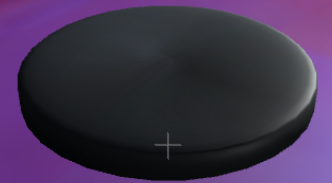
\includegraphics[scale = 1]{Check.png}

\textit{Figure 3 : Check-points}

\end{centering}

\newpage

\section{Réseau}

	\subsection{Interface (Thomas et Laurent)}

	\subsubsection{Serveur}
	
	\quad

Notre jeu utilise l’extension “Photon Network” de Unity, une extension complète et pratique pour gérer les connexions en réseau et hébergeant gratuitement un serveur suffisant pour notre jeu. Il gère automatiquement les serveurs du jeu et les “rooms” (la liste des différentes parties où les joueurs jouent), ce qui nous simplifie grandement la tâche. Photon Network héberge donc un serveur qui a pour but la gestion des rooms et de leurs joueurs, l’acceptation de connexion des clients, la connexion aux rooms, et le relais des informations entre les clients.
            

\quad

	\subsubsection{Client}

	\quad

Les clients utilisent donc Photon Network pour se connecter au serveur via une authentification. Cette authentification se fait en 2 temps. Premièrement client envoie son identifiant et son mot de passe sous forme chiffrée au serveur, ce dernier le chiffre d’une autre manière et le renvoie au client. Le client déchiffre avec la clé qu’il avait créée lors de son chiffrage et le renvoie au serveur. Le serveur ensuite n’a plus qu’à le déchiffrer avec sa propre clé pour pouvoir le comparer avec sa base de données et dit au client si l’authentification a réussi ou pas. Si elle a fonctionné le client peut après créer ou rejoindre une room et accéder à ses paramètres. Les joueurs ont accès à ces options via le menu multijoueur. Lorsqu’un client décide de créer une room, l’information est envoyée au serveur qui s’occupe de la créer, d’assigner le client en client maître, et de charger la scène. Ensuite les clients qui s’y connectent utilisent leur scène et récupèrent les données du client maître.
            

\quad

	\subsection{Synchronisation (Thomas et Laurent)}

	\subsubsection{Déplacement objets}

	\quad

La synchronisation des objets va s’effectuer sur une classe dédiée au multijoueur. Si l’objet déplacé est un personnage, c’est le client correspondant au personnage qui va envoyer la nouvelle position de celle-ci aux autres clients qui vont eux la modifier en local. Pour n’importe quel autre objet c’est le client maître qui va calculer les coordonnées puis les envoyer aux autres clients.

\quad


	\subsubsection{Instantiation}

	\quad

Le client qui souhaite instancier un objet va appeler la classe multijoueur pour que les instantiations se fassent en local sur chaque client.
\quad

	\subsection{Chat (Thomas et Laurent)}

	\quad

Notre jeu comporte un chat permettant aux clients de communiquer entre eux via une interface adéquate. Chaque message envoyé depuis un client est transféré au serveur qui identifie le client pour attribuer au message un pseudo et une heure d’envoi. Il est ensuite relayé aux autres clients, pour être finalement affiché dans leurs interfaces locales.



\quad

\newpage

\section{Gameplay}

	\subsection{HUD (Charles)}

	\quad

Ma partie principale lors de ce projet à été le développement de l'HUD (ou l'ATH), c'est ce que le joueur voit sur l'écran. Dans un premier temps, j'ai développé la barre de lucidité, c'est ce qui représente la vie du joueur. Dès que le joueur utilisera de la lucidité et par conséquent, la barre diminuera. Pour cela, j'ai crée trois images, une en noire qui représente le contour de la barre, une autre rouge qui représente le fond de la barre et enfin une troisième de couleur verte qui représente la lucidité. Cette dernière image diminue en jouant sur l'échelle de la position X entre 0 (barre vide) et 1 (barre pleine). La variation de la barre de lucidité est gérée par différents scripts.\\

J'ai ensuite créé le viseur que j'ai mis au centre de l'écran. Cela permet au joueur de pouvoir viser pour pouvoir lancer un clip (objet développé par Thomas) dans sa direction.\\


Je me suis aussi occupé de mettre en place différents textes qui permettent de donner des indications au joueur sur ce qu'il doit faire pour arriver au terme du niveau. A l'aide de différents scripts, lorsque le joueur effectue une action ou s'il se trouve dans une zone bien particulière, différents textes s'affichent en haut à droite de son écran pour l'aider dans son avancement.\\

Les deux textes sont synchronisés avec plusieurs scripts qui gérent l'affichage des textes, c'est-à-dire que lorsqu'un joueur fait une action spécifique, un message va envoyer une instruction au script lui disant d'afficher un texte spécifique, le script recevant ce message va donc afficher le texte sur l'écran du joueur.\\


Il y a aussi un texte en haut à droite qui permet au joueur de connaître ses objectifs pour accomplir le niveau et pouvoir en sortir. Dès qu'un joueur aura fini un objectif, l'objectif sera barré pour lui dire qu'il a accompli son objectif et qu'il peut passer au suivant, s'il y en a un. Les objectifs sont synchronisés dès que le joueur fait une action ou en finit un.\\


Les outils sélectionnées par le joueur sont visibles par l’HUD. Cela lui permet de savoir quelle arme il a en main. Des animations se feront dès que le joueur tirera. Si le joueur n’aura pas d’arme dans sa main, on verra juste une main qui lui permettra d’actionner les boutons et d’ouvrir les portes.\\


Ces outils seront sélectionnés à l’aide d’une roue d'armes où le joueur pourra sélectionner un outil qu’il souhaite utiliser comme le pistolet pour tirer les clips. Chaque outil apparaîtra dans la main du joueur. Le joueur pourra aussi ranger son outil pour qu’il puisse utiliser sa main. 

\quad

\quad

\quad

\begin{centering}

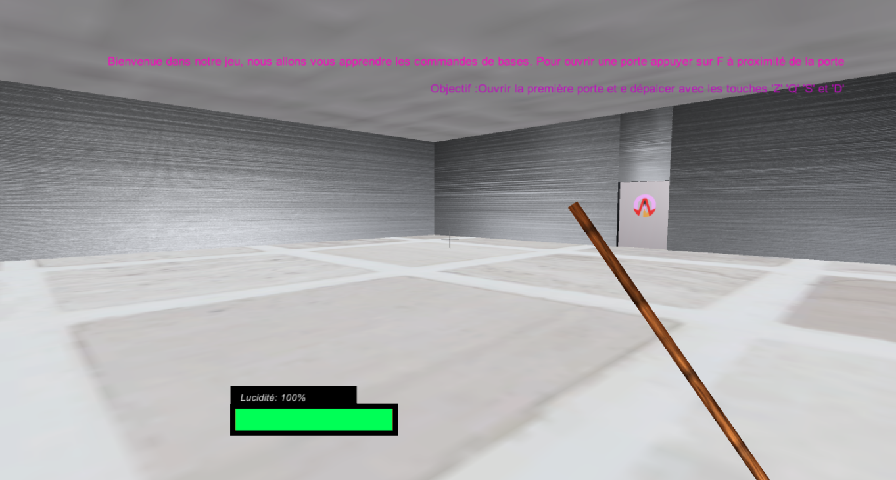
\includegraphics[scale = 0.65]{hud.png}


\quad

\textit{Figure 4 : HUD}

\end{centering}

	\quad

	\newpage


	\subsection{Menus (Charles)}

\quad

Menus : Le jeu possède deux types principaux de menus permettant aux joueurs différentes choses :\\

Les menus de sélection, comme le menu principal, le menu de sélection de niveau ou celui pour le multijoueur permettent principalement de sélectionner une scène à charger et se connecter au serveur pour rejoindre ou créer une room. \\

Les menus internes tels que le menu de pause et d’options qui permettent de quitter la partie actuelle, accéder aux réglages du jeu ou quitter le jeu.\\

Ces menus sont des interfaces utilisateur composées de boutons, textes, zones de saisie et barres de réglage.

\quad

\begin{centering}

\quad

\quad

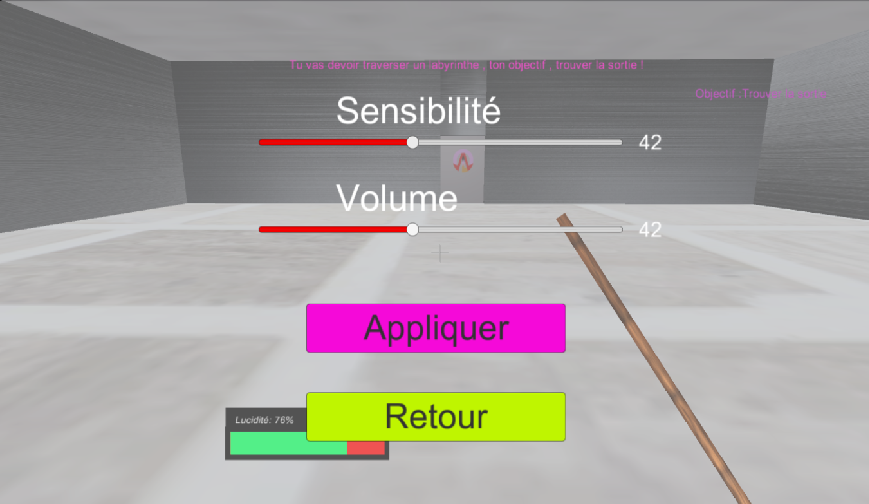
\includegraphics[scale = 0.65]{Menu_options.png}

\quad

\textit{Figure 5 : Le menu d'options}

\end{centering}

\newpage

		\subsubsection{Les objets interactifs}

	\quad

Nos niveaux comportent donc des épreuves dans lesquelles le joueur doit interagir avec des objets afin de faire son chemin vers la fin du niveau. Ces épreuves sont faites d’une suite d’objets dont voici quelques exemples :

\quad

		\subsubsection{La source de lucidité}

\quad

 C’est l’élément à la base de tout. Lorsque le joueur se situe à proximité de celle-ci, son stock de lucidité est rempli à son maximum. Son utilisation est illimitée mais sa présence est assez rare. On trouve donc des sources de lucidité uniquement à des endroits stratégiques, quand la lucidité du joueur commence à être faible.

	\quad

		\subsubsection{La porte}

	\quad

C’est le premier objet que le joueur rencontre en mode solo. La porte utilise un nombre fixe de lucidité du joueur pour être ouverte. Si le joueur meurt, toutes les portes précédemment ouvertes sont automatiquement refermées. Elles constituent l’élément de base du labyrinthe du premier niveau de solo.

\quad

		\subsubsection{La plateforme automatique}

	\quad

Ce sont des éléments mobiles permettant au joueur d’aller dessus pour rejoindre un endroit éloigné. Chaque plateforme effectue des cycles de mouvements entre deux points définis.

\quad

		\subsubsection{La plateforme guidée et les clips}

	\quad

Ces plateformes, contrairement aux dernières, sont guidées par le joueur grâce aux clips. Le joueur peut en effet lancer des clips destinés à guider la plateforme : le premier clip est envoyé sur un mur à l’endroit de destination voulu, et le second sur la plateforme à déplacer. Lorsqu’un joueur lance un clip, un nombre fixe de lucidité est enlevé au joueur.

	\quad

		\subsubsection{Le bouton}

	\quad

Les boutons permettent de dévoiler des objets masqués. Lorsqu’un joueur se trouve face à un bouton et appuie sur la touche de son clavier assignée à l’utilisation des boutons, d’autres objets sont dévoilés et un nombre fixe de lucidité est enlevé au stock du joueur.

	\quad


\newpage

\section{Son}

	\subsection {Musique (Charles)}

	\quad

Tout au long de jeu, j'ai inséré quelques musiques pour que l'ambiance soit plus vivante. Sous l'approbation des membres du groupe, j'ai défini différentes musiques pour les différents niveaux et aussi pour les différents menus. J'ai aussi fait en sorte que lorsque le joueur met le jeu sur pause, la musique se met automatiquement sur pause et reprend dès que le joueur clique sur le bouton "Reprendre".\\

Le but de la musique est qu'elle ne soit pas trop active (trop aggressive), elle doit être dans le style de jeu de réflexion, du coup je me suis plutôt tourné vers des musiques comme dans les salle d'attente donc je me suis interéssé aux musiques reposantes comme des musiques contenant l'instrument tel que le piano.\\

A l'aide du logiciel Audacity j'ai pu modifier certaines caractéristiques des différentes musiques que j'ai trouvé pour qu'elle soit le mieux adaptée au jeu. \\

En effet, il faut que la musique ne soit pas trop forte pour éviter qu’elle soit trop agressive ni qu’elle soit trop faible pour éviter que le joueur ne l’entende pas donc il a fallu trouver le juste milieu pour que la musique soit la meilleure possible.
De plus, il faut éviter que le musique soit trop forte sinon le joueur risque ne pas entendre les sons et qu’elle soit présente car si les sons se jouent seuls, ceci sera désagréable.

	\quad

\newpage

	\subsection{Les sons (Charles et Laurent)}

	\quad


 Je me suis occcupé d'insérer différents sons lorsque que le joueur fait des actions spécifiques comme quand le joueur avance, on entend un bruit de pas. Pour rendre possible tous ces sons, je me suis occupé de créer un gestionnaire qui contient tous les sons à des emplacements connus et à l'aide d'un script, dès que le joueur effectue une action, le script va recevoir un message avec le son à jouer, le script va l'éxecuter et le son sera joué.\\

Cette partie n'a pas été simple car il fallait que certains sons doivent se répeter sans qu'ils saturent (comme le bruit de pas si le joueur reste appuyé sur la touche pour avancer). J'ai du gérer aussi la désactivation du mode répeté pour éviter que les autres sons se jouent en boucle alors qu'ils ne devraient pas.\\

Le logiciel Audacity m'a une fois de plus été utile puisqu'il m'a permis d'enregistrer des sons mais aussi de les extraire et de modifier certains paramètres accoustiques qui permettent de le rendre de meilleure qualité. J'ai pu aussi extraire pas mal de sons des différentes séquences sonores que j'ai trouvé et je les ai raccourcis le plus possible pour éviter qu'ils ne soient en décalé avec l'action effectuée par le joueur.

\quad

\begin{centering}


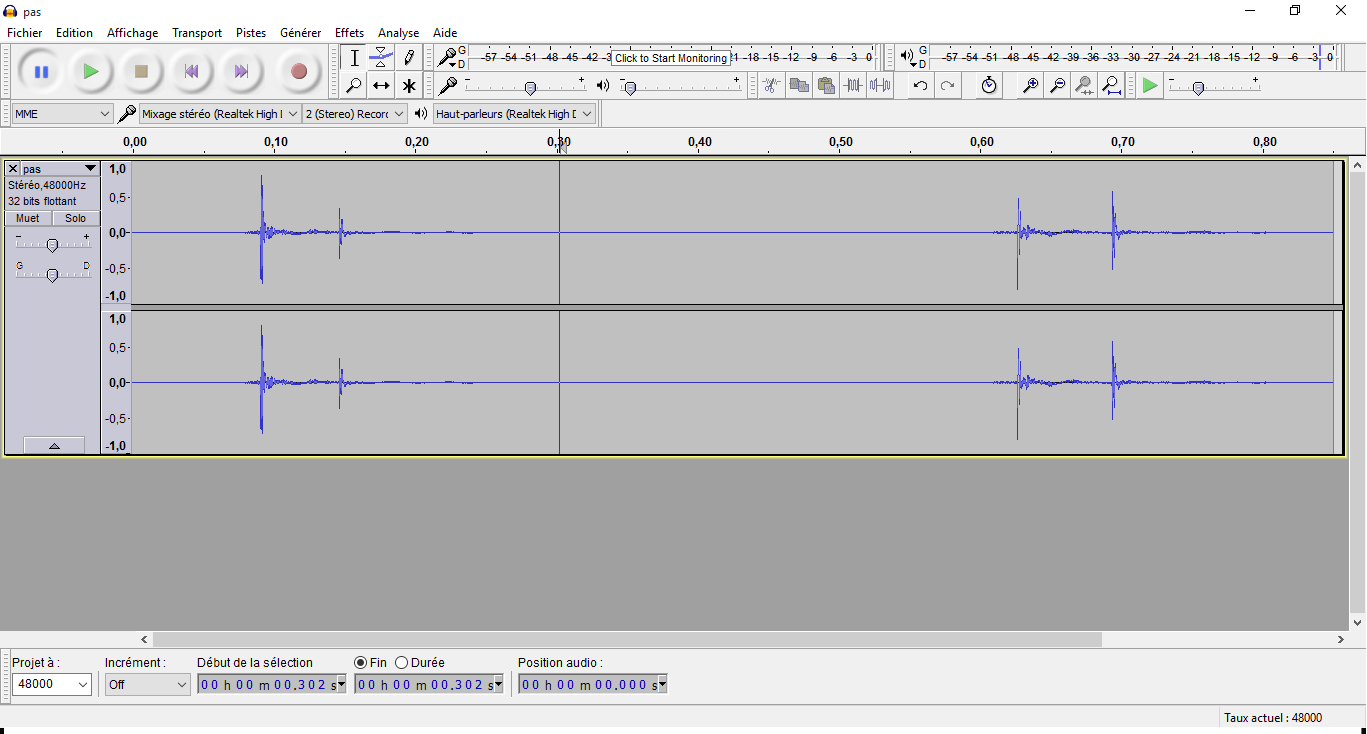
\includegraphics[scale = 0.35]{Audacity.png}

\textit{Figure 6 : Modification du son "Pas"}

\end{centering}

\newpage

\section{Site}


	\subsection{Conception (Laurent)}

	\quad

Notre site web a été créé entièrement sans modèle. Tout a été fait avec un éditeur de texte simple (Notepad++) permettant d’écrire du code php. On utilise donc le langage php pour l’affichage dynamique de données, et une base de données MySQL pour stocker ces données. Il a donc fallu apprendre comment manipuler des tables de données MySQL en php. Notre base de données contient 3 tables. Une première pour stocker les pseudos des utilisateurs, leurs mots de passe chiffrés, et leur niveau d'accès (pour différencier les utilisateurs des membres du projet pouvant ajouter des nouvelles). Une seconde contenant lesdites nouvelles, leurs auteurs et leurs dates, et une dernière table contenant les commentaires que les utilisateurs ajoutent sur la page de commentaires, leurs dates et leurs auteurs.

La base de données MySQL sert également à la connexion des utilisateurs à leur compte dans le jeu-même.

Le nom de domaine “lucidity.fr” nous appartient, correspondant au nom de notre jeu. Le site et la base de données sont hébergés sur un VPS (un serveur privé) donc il n’y a pas de risque de coupure comme auparavant quand il était hébergé sur un Raspberry Pi, sur un réseau domestique, et qu’il y avait des risques de coupure, et même un danger pour le réseau domestique de la personne.

\quad
\begin {centering}

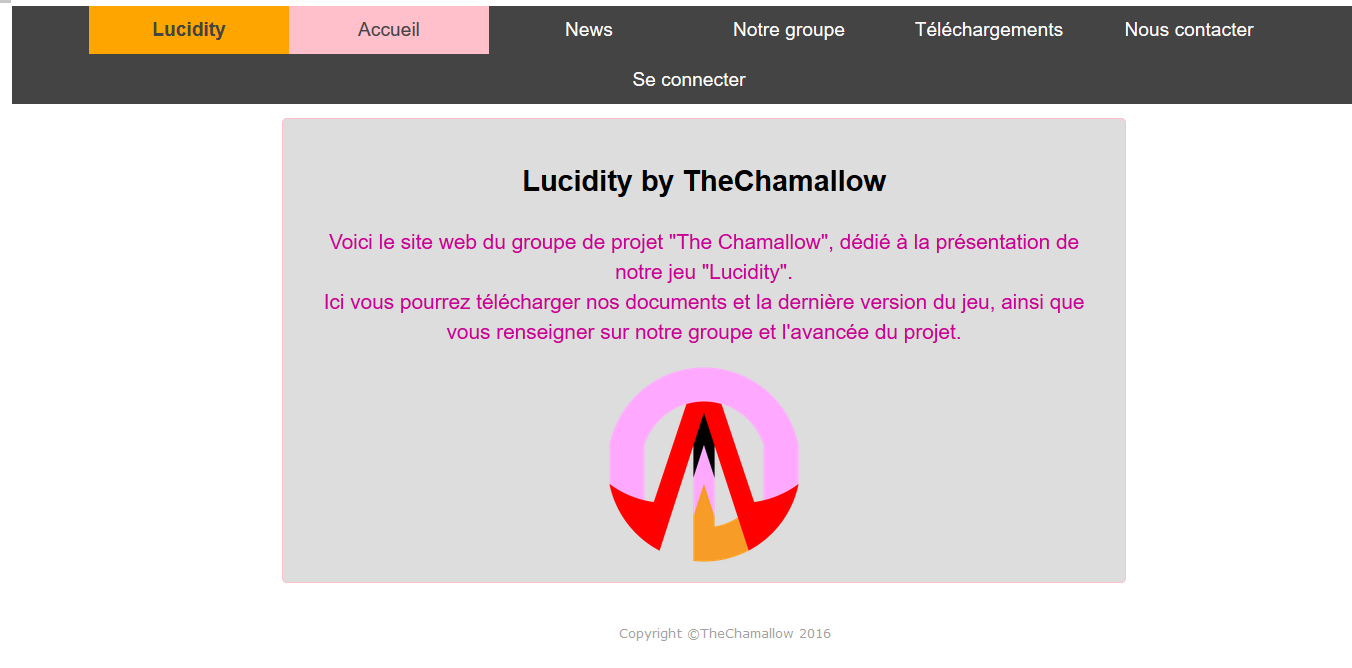
\includegraphics[scale = 0.35]{Le_site.png}

\textit{Figure 7 : Page d'accueil de notre site}

\end{centering}

\newpage

	\subsection{Utilisation (Charles)}

	\quad

Le site contient donc 6 pages : 
Une page principale présentant le site web. 

Une page de nouvelles sur laquelle les membres du groupe peuvent ajouter des nouvelles directement sur celle-ci quand ils sont connectés à leur compte.

Une page de présentation du groupe avec une présentation générale du groupe comme de l’origine du nom “The Chamallow”, et les présentations individuelles de chaque membre.

Une page de téléchargements contenant les différents documents (Cahier des charges, rapports, etc.) et, si l’utilisateur est connecté avec son compte, un lien de téléchargement de la dernière version du jeu.

Une page de contact sur laquelle les utilisateurs connectés peuvent poster publiquement des messages, afin qu’ils puissent nous faire des éventuelles remarques par rapport au jeu.

Une page de compte utilisateur. Par défaut, c’est une page sur laquelle les utilisateurs peuvent se connecter grâce à leur identifiant et leur mot de passe, ou créer un compte s’ils n’en possèdent pas. Une fois l’utilisateur connecté à son compte, cette page est une page personnelle sur laquelle il a accès à une autre page pour modifier son mot de passe.

Parallèlement, si l’utilisateur passe son curseur sur l’onglet de la dernière page, il voit se dérouler un onglet sur lequel il peut directement se connecter s’il ne l’est pas déjà, ou se déconnecter sinon.\\

Ce site est donc le support d’informations et de téléchargements du jeu. Il permet un contact entre les utilisateurs et les membres du groupe grâce aux pages de nouvelles et de commentaires. Il permet également à de nouveaux utilisateurs ne connaissant pas notre jeu de le découvrir, comme il s’est produit avec un utilisateur qui a changé “lucidity.com” en “lucidity.fr” et qui est donc arrivé sur notre site.\\

Chaque membre à un compte administrateur, c’est-à-dire qu’il peut éditer des news et supprimer des commentaires inappropriés.

\newpage

\section{Bénéfices et difficultés}

	\subsection{Bénéfices du projet}
	\quad

Ce projet a été bénéfique pour tout le groupe.
En effet, ce projet nous a permis d’avoir une première expérience sur ce que c’est que le travail en groupe.  \\

Cela a permis de développer l’entraide au sein du groupe, nous avons su faire confiance les uns aux autres que ce soit au niveau de l’implémentation des scripts qu’à la réalisation des différentes maps.\\

De plus, ce projet nous a permis d’accroître nos connaissances au niveau du code mais aussi d’avoir les bons réflexes quant à la réalisation d’un projet tel qu’un jeu.\\

Ce projet nous a aussi permis de partager nos connaissances entre les membres mais aussi d’en apprendre plus sur tous les points abordés dans le projet, Ainsi ce projet nous impose de savoir respecter des tâches et des horaires qui sont imposés et voir tous nos efforts récompensés par un jeu fonctionnel est très valorisant et est très encourageant pour la suite de nos études.


	\quad

\newpage

	\subsection{Difficultés rencontrées}

\quad
Comme tout projet, ce projet n’a pas été épargné par les difficultés de sa conception. En effet, les difficultés liées à sa conception ont été nombreuses et nous allons vous les présenter dans cette partie.\\

Pour commencer, ce projet a representé une grande quantité de travail que l’on devait fournir. Ce projet a pris beaucoup de notre temps durant ces derniers mois afin de le réaliser dans les temps. Pour y remédier, nous nous sommes beaucoup de fois rendus à EPITA le week-end ou pendant la semaine, si cette dernière était libre. Le groupe s’est beaucoup concerté quant à sa réalisation.\\

Ensuite, le réseau n’a pas été une partie de plaisir pour Laurent et Thomas, le plus dur a été d’adapter nos scripts disponibles en solo pour le multijoueur. Le multijoueur a dû modifier beaucoup de choses vu qu’il fallait prendre en compte plusieurs joueurs au lieu d’un, ce qui change totalement les scripts.\\

Une de nos principales difficultés a été de trouver des idées pour nos maps pour éviter que les maps soient similaires et donc trop répétitives pour le joueur. Nous avons eu des difficultés à trouver des élements à mettre dans nos maps mais aussi comment le joueur fera pour arriver à la fin du niveau en ayant un minimum réfléchi. Pour trouver nos idées, tout le groupe s’est mis à réfléchir sur différents éléments que l’on pourrait ajouter tout au long des niveaux pour réaliser des maps originales.\\

Evidemment, qui dit réflexion à plusieurs, dit concertation. Le plus compliqué dans cette étape est que l’on soit tous d’accord et cela n’a pas été chose facile puisque chaque membre du groupe avait un avis différent sur la chose et ce qui donnait quelques confrontation mais au final le groupe a pu se mettre d’accord sur tous les élements qui sont actuellement dans nos différends niveaux.\\

\newpage

Trouver une histoire n’a pas été simple non plus puisqu’il fallait qu’on se mette d’accord sur l’histoire mais aussi que cette dernière soit cohérentes avec le jeu. Chaque membre a eu des idées mais le plus dur a été de se mettre d’accord sur les idées de chacun. L’histoire a mis du temps à venir mais elle est bien là.\\



Après avoir trouvé les idées, il faut les mettre en place mais cela n’a pas été de tout repos car il fallait aussi bien les mettre sur les maps que les implémenter au niveau du script. Cela nous a rajouté du temps de travail mais pour un résultat qui vaut le coup.\\

Enfin, lorsque l’on modifie quelque chose, on a souvent des répurcussions sur les autres objets et du coup on doit souvent passer en revue tous les objets si on en modifie un, pour vérifier qu’il n’y ait pas de problèmes notamment sur la synchronisation des plateformes.

\quad 

\newpage

\section{Bilan personnel}

\subsection{Marion CLAUS}

\quad

Ce projet représente énormément de choses pour moi puisque c’est la première fois que je fais un projet aussi grand en groupe. C’est donc une nouvelle expérience très enrichissante tant sur le plan personnel que le plan professionnel.\\

Bosser sur ce projet m’a beaucoup enseigné sur le travail de groupe. Les deux choses qu’il me semble indispensable quand l’on travaille à plusieurs est de pouvoir compter sur nos coéquipiers, savoir qu’ils sont prêts à nous aider si on a un problème, ainsi que la communication qui permet que le groupe soit organisé et donc d’avoir une meilleure efficacité dans notre travail.\\

Ce projet m’a aussi appris beaucoup de choses sur le graphisme puisque je me suis surtout occupée de cette partie, ainsi que réussir à gérer les différentes tâches que j’avais à faire par rapport à l’emploi du temps qu’on a donné pour les soutenances dans le cahier des charges.\\

 Mon objectif pour ce projet était de faire un jeu dont nous pourrions être fiers et pour un premier projet, je suis satisfaite de ce que nous avons fait, et heureuse que le jeu soit enfin fini. J’ai beaucoup aimé travailler avec mon groupe, il y avait une ambiance agréable bien que des fois il a été dur de mettre tous les membres du groupe d’accord. 

\newpage

\subsection{Thomas DELECROIX}

\quad


Ce projet du deuxième semestre à Epita fut mon premier projet en groupe ce qui représentait déjà une grosse implication au niveau individuel pour le travail de groupe. Avant cela je n’avais jamais utilisé Unity, et j’avais tout à apprendre. Chaque personne du groupe a dû s’engager personnellement dans ce projet parce qu’on ne pouvait pas se permettre de travailler avec un seul membre en moins, on était tous utile au projet. On avait donc chacun une responsabilité vis à vis du groupe, on avait tous quelque chose à apporter au groupe et le travail mal fait pouvait déteindre sur celui-ci.\\

En plus de cela j’étais également chef de projet, ce qui entraînait beaucoup de responsabilités de ma part. En tant que tel j’ai du m’occuper des relations humaines qui sont à la base d’un groupe. J’ai donc appris à gérer plusieurs situations et problèmes en même temps. Pendant toute la durée du projet il a fallu garder le groupe soudé et uni pour arriver sur un jeu abouti sur lequel nous avions tout donné.\\

Au niveau de mes connaissances personnelles cela m’a permis de progresser énormement, au tout début je ne savais pas du tout utiliser Unity mais au fur et à mesure que j’ai regardé des tutoriels j’ai commencé à prendre le logiciel en main. Même si j’ai rencontré des difficultés j’ai réussi développer les scripts petit à petit et j’ai appris à résoudre mes problèmes.\\

Au final ce projet m’a permis de m’ouvrir aux autres, d’échanger avec eux mes connaissances ainsi que d’en recevoir. Néanmoins je suis content de la tournure que le projet a pris et de sa finalisation. Ce fut une expérience positive dont je me souviendrai et garderai de bons souvenirs.

\newpage

\subsection{Charles GINANE}

\quad

Au début du projet, je suis parti confiant. Je savais que nous formions un bon groupe et que nous allions bien avancer ensemble. Je suis parti avec peu de connaissances dans le domaine de la programmation d’un jeu et du travail en groupe sur un projet quelconque. 
Grâce à mon premier projet, j’ai pu avoir pas mal de connaissances sur le domaine de la programmation mais aussi sur ce que représente le travail en groupe.\\


Je me suis beaucoup rendu utile tout au long du projet, effectué des tâches concrètes à l’aide des connaissances en code que j’ai acquis tout au long de mon année à EPITA.\\


Sur certains points je ne me sentais pas à l’aise voire même je pensais ne pas y arriver et maintenant j’y arrive sans aucun problème. C’est surtout les autres membres du groupe qui m’on permis de prendre confiance en moi tout au long de ce projet en m’aidant lorsque j’étais en difficulté ou en me faisant confiance sur certaines tâches à accomplir. \\


Ce projet m’a aussi permis de savoir comment faire pour résoudre certains problèmes dans le code mais aussi à montrer mon opinion face à des décisions de groupe comme pour le choix des textures. 
J’ai su prendre des initiatives sur mes responsablilités afin d’optimiser mon travail et aussi de prendre du recul sur le travail afin de réussir le mieux possible ma tâche.\\

Je suis fier du travail fourni par l’ensemble du groupe puisque nous avons en résultat un jeu fonctionnel qui respecte entièrement notre cahier des charges et que nous avons fini dans les temps. Il y a eu une très bonne cohésion au sein du groupe.\\


Ce projet a été une bonne expérience pour moi puisqu’il m’a permis de savoir ce qu’il faut faire et ce qu’il ne faut pas faire pour le développement de futurs projets au sein de l’école mais aussi au sein d’un milieu professionnel .
J’ai pu en apprendre sur moi-même et adapter ma façon de travailler pour travailler le plus efficacement possible.\\

J’ai aussi amelioré mon oral en étant volontairement deux fois chef de soutenance ce qui m’as permis, une fois de plus, de prendre confiance en soi et d’être apte à parler devant un public sans problème.\\

Selon moi, ce premier projet est très instructif puisqu’il nous a permis d’avoir une première application concrète sur ce qu’on a appris en programmation mais aussi de respecter un cahier des charges, de respecter des horaires et aussi de tenir compte de l’avis des autres. Ce projet m’a été très encourageant quant à la suite de ma scolarité au sein de l’EPITA et des autres projets que nous devrons réaliser ultérieurement.

\quad



\subsection{Laurent MARCHAUD}

\quad

La réalisation de ce projet fut très enrichissante tant sur le point de vue humain que sur celui de l’apprentissage.\\

Avant de commencer le développement du jeu, je pensais que j’aurais du mal à bien utiliser Unity, mais l’apprentissage a été constant, j’ai beaucoup appris de moi-même ou en suivant des tutoriels sur Internet. Ce qui est bien avec Unity, c’est que beaucoup de personnes l’utilisent donc lorsque quelqu'un rencontre des problèmes, il en fait part sur des forum d’entraide pour que d’autres développeurs lui viennent en aide. Les forums sont donc remplis d’informations très utiles, facilement retrouv ables en faisant une simple recherche sur Google.\\

\newpage


J’ai donc appris l’autoformation, ce qui ne peut qu’être positif pour la suite, notamment pour l’apprentissage de développement dans d’autres langages de programmation.\\

Sur le plan social, le projet a appris à chaque membre du groupe à s’adapter à l’organisation de chacun, à accepter les choix des autres.\\

Il était nécessaire de travailler régulièrement, notamment pendant notre temps libre les weekends, ce qui n’a pas été un problème pour moi, j’ai même apprécié les périodes de travail intensif, motivantes bien que fatiguantes.\\

Je suis assez fier du résultat final et du travail fourni tout au long de ce semestre pour créer notre jeu. \\

Je pense que si c’était à refaire, notre groupe irait beaucoup plus rapidement puisque nous avons maintenant tous de bonnes connaissances en Unity. En effet, nous avons perdu beaucoup de temps au tout début puisque nous n’avions aucune connaissance en Unity donc nous avons tous commis des erreurs qu’il a fallu rectifier par la suite.


\quad

\newpage
 
\section{Conclusion}

\quad

nous avons pu former un groupe de travail soudé, motivé et efficace. Malgré les difficultés rencontrées lors des périodes de travail, nous avons su rester unis pour des sessions efficaces de développement et de rédaction. Chaque soutenance nous a permis de nous situer par rapport à l’avancement du projet, les éventuelles améliorations que l’on devait apporter, mais surtout, cela nous motivait plus que tout pour la suite. 

Chaque membre du groupe avait sa spécialité dans le développement du jeu, nous étions tous complémentaires. Il a donc fallu que chaque membre gagne la confiance des autres et fasse ses preuves pour que l’on avance efficacement et en toute confiance. 

L’aboutissement de ce projet était un objectif commun au groupe, pour lequel tout le monde a dû s’impliquer, qui a plus que soudé le groupe, formant ainsi une vraie équipe prête à faire face à tout éventuel problème. Ce qui nous a permis d’arriver à terme de ce projet était la cohésion et la bonne entente entre chaque membre du groupe. Au final nous avons pu conclure ce projet en étant toujours fiers du travail que nous avions fourni. Le développement d’un jeu est une étape que tout passioné d’informatique doit subir car elle révèle différentes problématiques, pouvoir le réaliser en groupe cette année a été une merveilleuse expérience et nous ne sommes pas mécontents de l’avoir faite. Les progrès que nous avons fait étaient inimaginable au début du projet mais nous avons quand même travaillé et nous nous sommes acharnés sur celui-ci pour obtenir le meilleur compromis. Le groupe The Chamallow a à présent fini de développer le jeu Lucidity, que nous avons eu l’honneur de vous présenter, mais nous sommes bien loin d’oublier ce que cette expérience nous a apporté. 
\quad

\newpage

\section{Webographie}

\underline{\textbf{Unity :}}

Unity, Unity manual. Unity, 2016 :


\url{http://docs.unity3d.com/Manual/index.html}

\quad

Unity, Unity answer. Unity, 2016 :


\url{http://answers.unity3d.com/}

\quad

Microsoft, MSDN. Microsoft, 2016 :


\url{http://msdn.microsoft.com/}

\quad


\underline{\textbf{Graphique :}}

Yojigraphics, Belender 2.6 texturing personnage partie 1, YouTube, 29 Juin 2012 : 

\url{https://www.youtube.com/watch?v=JQCrGldir6k}

\quad

designtuto, Modéliser un personnage avec Blender, YouTube, 1 Février 2011 :


\url{https://www.youtube.com/watch?v=4Z5IsdPj2Rg}

\quad

\underline{\textbf{Réseau}}

Quill18creates, Multiplayer First-Person Shooter, YouTube, 2 Juillet 2014:


\url{https://www.youtube.com/playlist?list=PLbghT7MmckI7BDIGqNl_TgizCpJiXy0n9}

\quad

Exit Games, Photo Unity 3D networking, Photon, 2016 


\url{https://www.photonengine.com/en/PUN}

\quad

Exit Games, Photon Unity networking intro, Photon, 2016


\url{https://doc.photonengine.com/en-us/pun/current/getting-started/pun-intro}

\quad

\newpage

\underline{\textbf{Son}}

RogueLike, Unity - Audio and Sound manager. Unity, 2016 :


\url{https://unity3d.com/learn/tutorials/projects/2d-roguelike-tutorial/audio-and-sound-manager}

\quad

Abhinav a.k.a Demkeys, Unity Tutorial: Audio Manager, YouTube, 23 Juin 2014 :


\url{https://www.youtube.com/watch?v=yIT0ontYzpk}

\quad

\underline{\textbf{Gameplay}}

Unity, Health HUD, Unity, 2016 :


\url{https://unity3d.com/learn/tutorials/projects/survival-shooter/health-hud}

\quad

\newpage

\section{Remerciements}

\quad

Nous profitons de ce rapport de projet pour passer nos remerciements à différentes personnes qui nous ont aidé tout au long de ce projet, que ce soit directement ou indirectement\\

Nous voudrions déjà remercier les professeurs de notre école, notamment les ceux d’algorithmique, qui ont permis l’organisation de ce projet en première année qui est une chose très intéressante et surtout un entraînement pour la vie professionnelle plus tard.
Nous remercions également l’association GConfs et nos ACDC qui ont fait une soirée spéciale pour débuter le projet ainsi que un TP pour nous apprendre Unity.\\

Nous remercions aussi les personnes qui ont joué à notre jeu qui ont pu nous donner des conseils auxquels nous n’aurions jamais pensé. Nous remercions donc 
Jérome LEFEVRE, Coline PICARD, Laurie RIGAL, Alan ROBLEDILLO

\quad

\newpage

\section{Annexe}

\begin {centering}

\quad


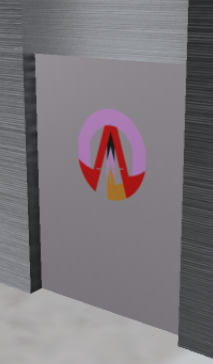
\includegraphics[scale = 0.3]{Porte.png}

\quad

\textit{Figure 8 : porte présente dans nos niveaux}

\quad

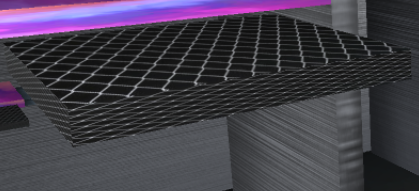
\includegraphics[scale = 0.5]{Plateforme.png}

\quad

\textit{Figure 9 : Une plateforme automatique}

\quad

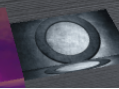
\includegraphics[scale = 0.5]{Plateforme2.png}

\quad

\textit{Figure 10 : Plateforme controlée par les clips}

\quad


\includegraphics[scale = 0.5]{Bouton.png}

\quad

\textit{Figure 11 : Bouton présent dans le niveau 2 du solo}

\end{centering}
\end{document}